\section{Design and construction}\label{sec:design}
\sectionstate{partial}{\texttt{docs/detector\_spec/spec.py} (97 numbers, 9 unknown, 31 assumed);
spec page \texttt{notes/mx17-detector-spec.html}; Gerber files; PLAN\_38 (charge balance)}
\intent{A complete, citable description of the MX17 module, layer by layer, and of how it was built and
qualified. Most of this section is Stephan's: the production side is not in our analysis repository.}

\subsection{Chamber layout}
\tbw{Entrance window and flange, 30\,mm drift gap, cathode, field cage. Active area; measured efficient area
$399.4\times359.9$\,mm$^2$.}
\askStephan{Field cage: number of ring strips per board, pitch and width, resistor chain. Was chamber B's field cage missing or damaged?}
\askStephan{Window: 60\,\textmu m mylar? aluminised on one side or both, Al thickness, which side faces the gas.
Cathode: 50\,\textmu m kapton with copper on one side, copper thickness. Operating overpressure / window bulge;
is the drift gap exactly 30.0\,mm at the centre under pressure?}

\subsection{Amplification stage and resistive layer}
\tbw{Bulk Micromegas: mesh, amplification gap, pillars. Resistive strips over the pads, insulator, how the charge
reaches the pads (capacitive coupling through the insulator).}
\askStephan{Mesh: material, wire diameter, opening, thickness, supplier; calendered, and its thickness after?
Amplification gap 150\,\textmu m? photoresist and number of laminations; pillars \O\,0.6\,mm on a 4.68\,mm grid?}
\askStephan{Resistive strips: width and pitch (550/800\,\textmu m, while the readout pitch is 780\,\textmu m?), direction,
number; thickness after curing; paste grade and supplier; sheet resistance or end-to-end resistance (any measurement on these boards?);
the insulator between strips and pads (kapton thickness, adhesive type and thickness).}

\subsection{Readout board}
\tbw{512\,$\times$\,512 square pads (0.68\,mm on a 0.78\,mm pitch) on L4, each connected by a via to an X strip (L6) or a
Y strip (L5). Connectors, DREAM front-end, channel count.}
\askStephan{Confirm the readout scheme and which pads go to which view. Is there a stack-up drawing
(layer order, copper and dielectric thicknesses)? Behind the board: Rohacell grade and the back mylar.}
\askStephan{We measure a $\sim$19\,mm dead band at each end of Y on every chamber. Is that the covered copper bus
where the resistive strips are terminated?}

\begin{figure}[t]
  \centering
  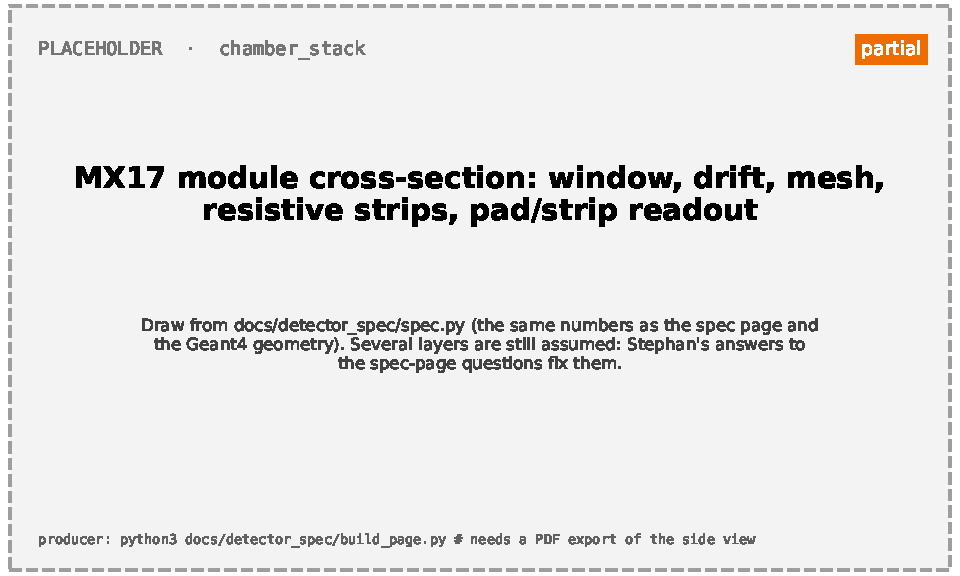
\includegraphics[width=0.9\linewidth]{chamber_stack}
  \caption{\tbw{Cross-section of the MX17 module, to scale in $z$ for the amplification region.}}
  \label{fig:stack}
\end{figure}
\begin{figure}[t]
  \centering
  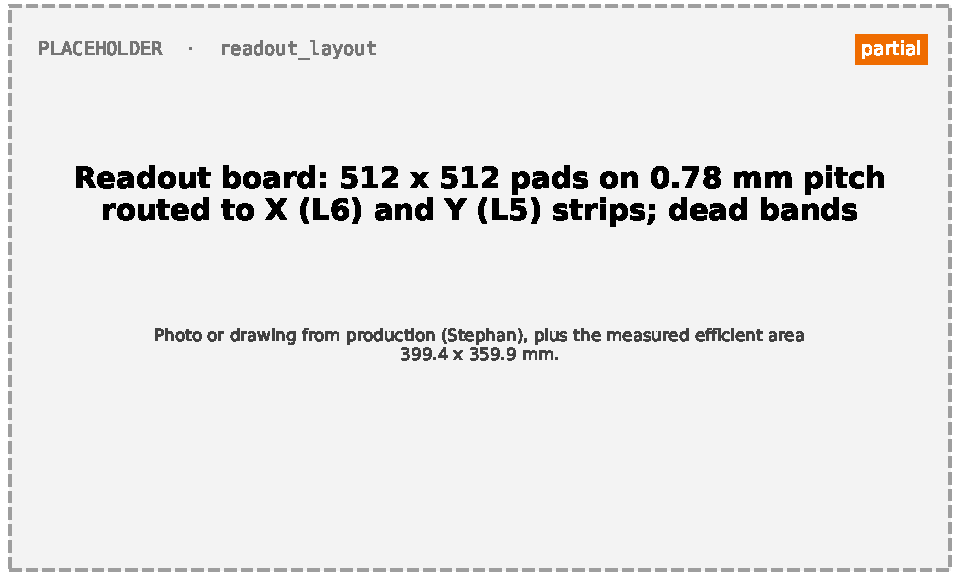
\includegraphics[width=0.8\linewidth]{readout_layout}
  \caption{\tbw{Readout board: pad pattern, X/Y routing and the dead bands.}}
  \label{fig:readout}
\end{figure}

\subsection{Production and quality control}
\tbw{How many boards were built, where and when; the bulk process; the resistive-layer printing; acceptance tests
(resistance mapping, HV training, leak and gas tightness, gain uniformity). Which board went into which chamber.}
\askStephan{This subsection is yours: production sequence, QA steps and their results, and anything that
distinguishes the boards of det2, det3, det4, det6 and det7 (in particular the det4 board, \cref{sec:det4}).}
